\documentclass[handout]{beamer}

\usepackage[utf8]{inputenc} % Language and font encoding
\usepackage[icelandic]{babel}
\usepackage[T1]{fontenc}


\usepackage{tikz}
\usepackage[listings,theorems]{tcolorbox}
\usepackage{booktabs}
\usepackage{minted} %Minted and configuration
\usemintedstyle{default}

\renewcommand{\theFancyVerbLine}{\sffamily \arabic{FancyVerbLine}}
%%%%%%%%%%%
% More math
%%%%%%%%%%%
\newcommand{\Mod}[1]{\ \text{mod}\ #1}

%%%%%%%%%%%%%%%%%%%%%%
% Beamer configuration
%%%%%%%%%%%%%%%%%%%%%%
\setbeamertemplate{navigation symbols}{}
\usecolortheme{dove}
\setbeamercolor{frametitle}{fg=white}

\usebackgroundtemplate%
{%
\vbox to \paperheight{

\includegraphics[width=\paperwidth]{Pics/hi-slide-head-2016}

\vfill
\hspace{0.5cm}
\includegraphics[width=0.3\paperwidth]{Pics/hi-von-logo}
\vspace{0.4cm}
    }%
}

\AtBeginSection[]
{
  \begin{frame}<beamer>
    \frametitle{Yfirlit}
    \tableofcontents[currentsection]
  \end{frame}
}

\setbeamerfont{frametitle}{size=\normalsize}
\addtobeamertemplate{frametitle}{}{\vspace*{0.5cm}}

%%%%%%%%%%%%%%%%%%%%%%%%%
% tcolorbox configuration
%%%%%%%%%%%%%%%%%%%%%%%%%

% Setup from: http://tex.stackexchange.com/a/43329/21638
\tcbset{%
    noparskip,
    colback=gray!10, %background color of the box
    colframe=gray!40, %color of frame and title background
    coltext=black, %color of body text
    coltitle=black, %color of title text 
    fonttitle=\bfseries,
    alerted/.style={coltitle=red, colframe=gray!40},
    example/.style={coltitle=black, colframe=green!20, colback=green!5},
}


%%%%%%%%%%%%%%%%%%%%%%%
% Further configuration
%%%%%%%%%%%%%%%%%%%%%%%
\hypersetup{colorlinks=true,pdfauthor={Eirikur Ernir Thorsteinsson},linkcolor=blue,urlcolor=blue}
\graphicspath{{./Pics/}}

\author{Eiríkur Ernir Þorsteinsson}
\institute{Háskóli Íslands}
\date{Haust 2016}

\title{Stærðfræðimynstur í tölvunarfræði}
\subtitle{Vika 4, fyrri fyrirlestur}

\begin{document}

\begin{frame}
\titlepage
\end{frame}


\section{Inngangur}

\begin{frame}{Í síðasta tíma}
\begin{itemize}
 \item Stöðvunarvandamálið
 \item Vöxtur falla
 \begin{itemize}
  \item Stóra O ritháttur
  \item Aðrir rithættir - $\Theta$, $\Omega$
 \end{itemize}
\end{itemize}
\end{frame}

\begin{frame}{Leiðrétting!}
Í heimadæmum 3, spurningu 2 er sýnd stígandi runa:
\[
 c_1 = 1, c_2 = 5, c_3 = 10, c_4 = 25
\]
Til samræmis við reiknirit á glærum og í bók ætti runan að vera lækkandi:
\[
 c_1 = 25, c_2 = 10, c_3 = 5, c_4 = 1
\]
\end{frame}

\section{Reikniflækja}

\begin{frame}{Reikniflækja}
\begin{itemize}
 \item Höfum lýst því hvernig hægt er að nota stóra-O rithátt til að tákna vöxt falla
 \item Notum nú föll til að tákna hegðun reiknirita
 \item Getum táknað hegðunina með falli af inntaksstærð reikniritsins
 \begin{itemize}
  \item Sé reiknirit að vinna með inntak af stærð $n$ getum við táknað ákveðna hegðunareiginleika þess með falli $f(n)$
 \end{itemize}
 \item Talað er um reikniflækju eða lausnarflækjustig (e. \emph{computational complexity})
\end{itemize}
\end{frame}

\begin{frame}{Reikniflækja}
\begin{itemize}
 \item Skoðum fyrst og fremst tímaflækju (e. \emph{time complexity}) reiknirita
 \begin{itemize}
  \item Lýsum keyrslutíma reiknirits sem falli af inntaksstærð
  \item Venjulega er keyrslutímafallið síðan sett fram með stóra-O eða stóra-$\Theta$ rithætti
 \end{itemize}
 \item Einnig er til minnisflækja (e. \emph{space complexity})
 \begin{itemize}
  \item Ekki fjallað um í bók, sleppum
  \item Minnisflækja og tímaflækja eru tengd - til að skrifa í minni þarf tíma
 \end{itemize}
\end{itemize}
\end{frame}

\begin{frame}{Tímaflækja}
\begin{itemize}
 \item Til að kvarða tímaflækju reiknirits eru grunnaðgerðir þess taldar
 \begin{itemize}
  \item Dæmi um grunnaðgerðir: Breyta búin til, samlagning tveggja talna, samanburður á breytum
 \end{itemize}
 \item Fallið sem lýsir keyrslutíma er þá í raun fall sem lýsir fjölda grunnaðgerða
 \item Varnagli: Tímaflækja hunsar ýmis praktísk atriði sem koma við sögu í raunverulegum tölvum
 \begin{itemize}
  \item Minni er ekki allt jafn hraðvirkt
  \item Grunnaðgerðir taka mis langan tíma
 \end{itemize}
\end{itemize}
\end{frame}

\begin{frame}{Tímaflækja max reikniritsins}
Lítum aftur á \texttt{max} reikniritið. Hver er tímaflækja þess á $\Theta$-sniði?

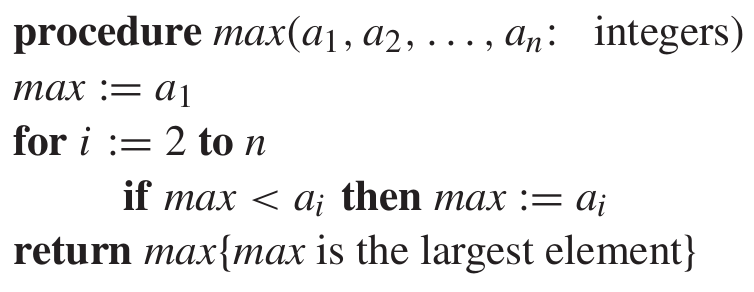
\includegraphics[width=\linewidth]{max-element} \pause

Alltaf þarf að gefa hágildinu upphafsgildi og skila. Fyrir hvern lið í rununni þurfum við að framkvæma tvo samanburði. Í eitt eða fleiri skipti þarf að uppfæra hágildið. Tímaflækjan er $\approx 2n$ sem er $\Theta(n)$.
\end{frame}

\begin{frame}{Versti- besti og meðalkeyrslutími}
\begin{itemize}
 \item Keyrslutími reiknirita er oft mismunandi eftir gerð inntaka
 \item Þá setjum við fram keyrslutíma fyrir mismunandi tilfelli
 \item Mikilvægasta tilfellið er oftast versti keyrslutíminn (e. \emph{worst-case complexity})
 \item Önnur tilfelli eru meðalkeyrslutími (oft erfitt að reikna) og besta tilfellið (oft lítið gagn í þeim upplýsingum)
 \item Athugum að rugla ekki saman hugtökunum um efri og neðri mörk á vexti falla og hugtökunum um besta og versta keyrslutíma
\end{itemize}
\end{frame}

\section{Tímaflækjur ýmissa reiknirita}

\subsection{Leitarreiknirit}

\begin{frame}{Línuleg leit}
Upprifjun: Línuleg leit

\begin{center}
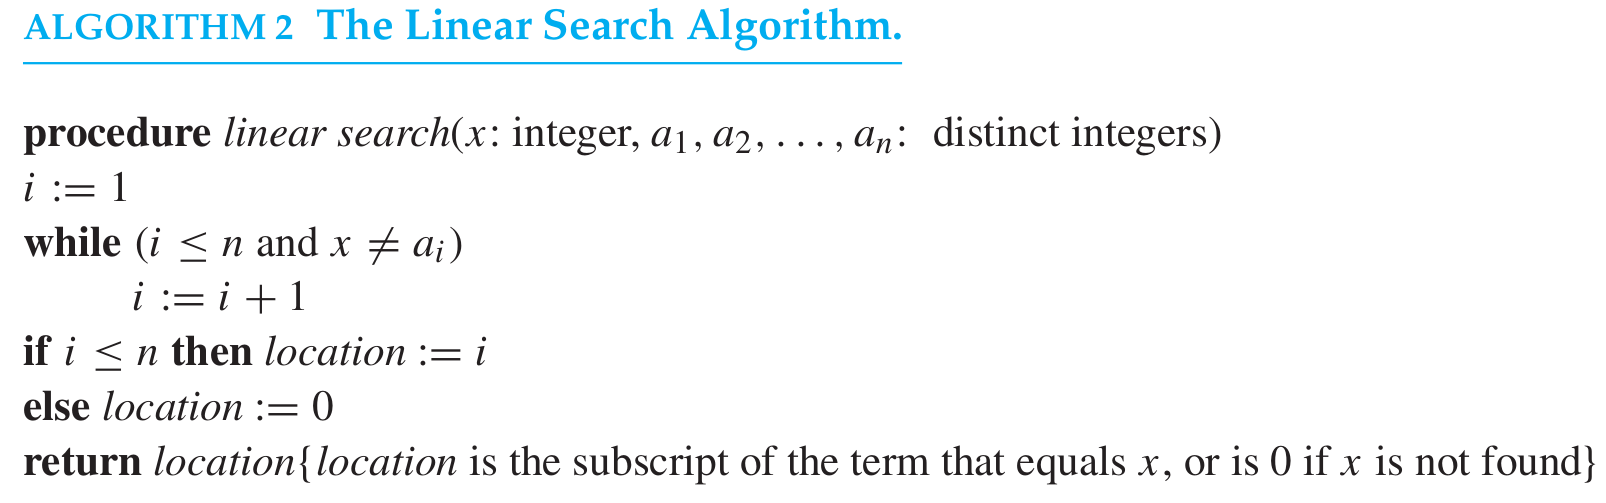
\includegraphics[width=\textwidth]{linear-search}
\end{center}
\end{frame}

\begin{frame}{Versti og besti keyrslutími}
\begin{itemize}
 \item Dæmi: Línuleg leit þarf mjög mismunandi tíma
 \item Keyrslutíminn fer eftir staðsetningu liðarins sem leita á að
 \begin{itemize}
  \item Versta tilfellið: Liðurinn er ekki til eða úti á enda, þurfum að skoða alla \pause
  \begin{itemize}
   \item $\Theta(n)$
  \end{itemize}
  \item Besta tilfellið: Liðurinn er fremst í rununni \pause
  \begin{itemize}
   \item $\Theta(1)$
  \end{itemize}
  \item Meðaltilfellið: Jafn líklegt að liðurinn sé hvar sem er \pause
  \begin{itemize}
   \item $\Theta(n)$
  \end{itemize}
 \end{itemize}
\end{itemize}
\end{frame}

\begin{frame}{Helmingunarleit}
Upprifjun: Helmingunarleit

\begin{center}
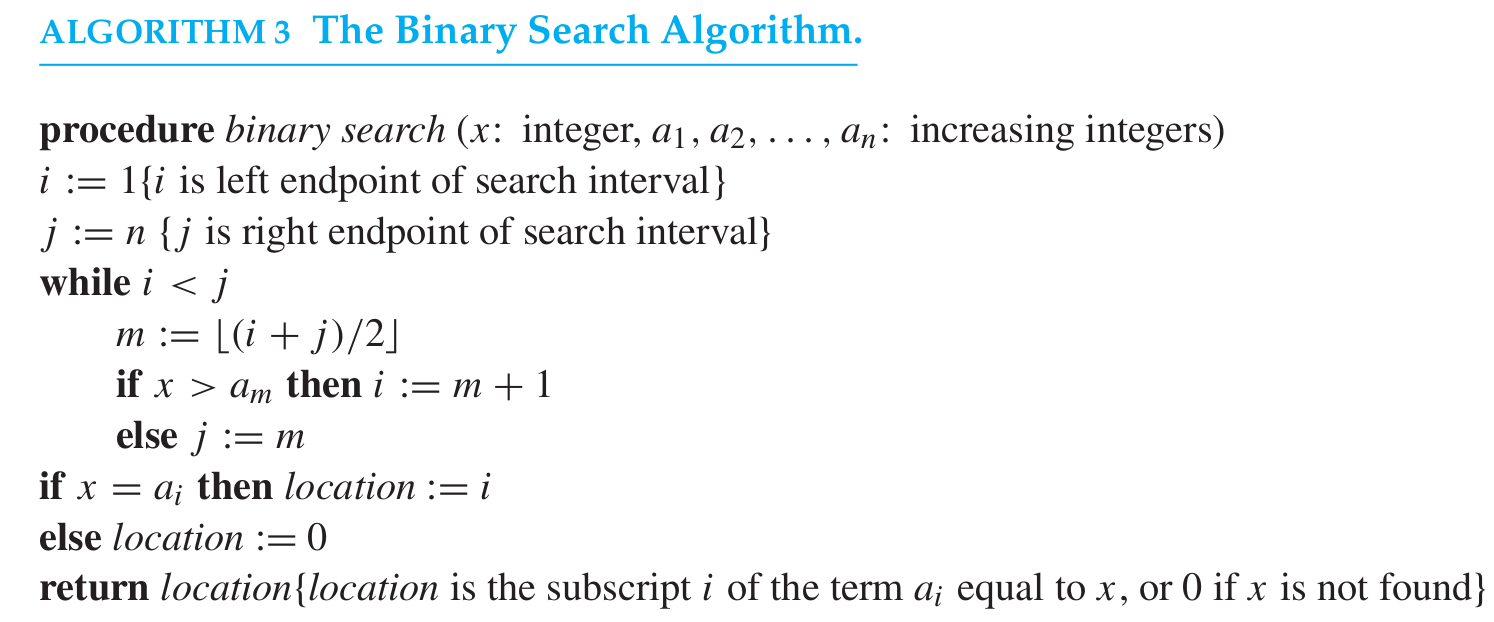
\includegraphics[width=\textwidth]{binary-search}
\end{center}
\end{frame}

\begin{frame}{Tímaflækja helmingunarleitar}
\begin{itemize}
 \item Gerum ráð fyrir að lengd rununnar sem helmingunarleit á að leita í sé $n = 2^k$ þar sem $k \in Z^+$
 \begin{itemize}
  \item Sé lengd rununnar ekki veldi af $2$ gerum við ráð fyrir að um sé að ræða hlutrunu í lengri runu 
 \end{itemize}
 \item Leitarbilið minnkar niður í stærð $2^{k-1}$ eftir fyrstu ítrun, $2^{k-2}$ eftir aðra ítrun\ldots
 \item Fastur fjöldi aðgerða í hverri ítrun \pause
 \begin{itemize}
  \item Þurfum $k$ skref og $n = 2^k$, svo um er að ræða $\Theta(\log(n))$ reiknirit
 \end{itemize}
\end{itemize}
\end{frame}

\begin{frame}{Lograr í tímaflækjum}
Í tölvunarfræði fáumst við oftast við logrann með grunntöluna 2. Grunntalan skiptir ekki máli í stóra-$\Theta$ framsetningu (og tengdum ritháttum) vegna þess að lograr eru fast margfeldi hver af öðrum.

\[
 \log_b(x) = \frac{\log_k(x)}{\log_k(b)}
\]

\end{frame}

\subsection{Röðun}

\begin{frame}{Innsetningarröðun}
Upprifjun - innsetningarröðun
\begin{center}
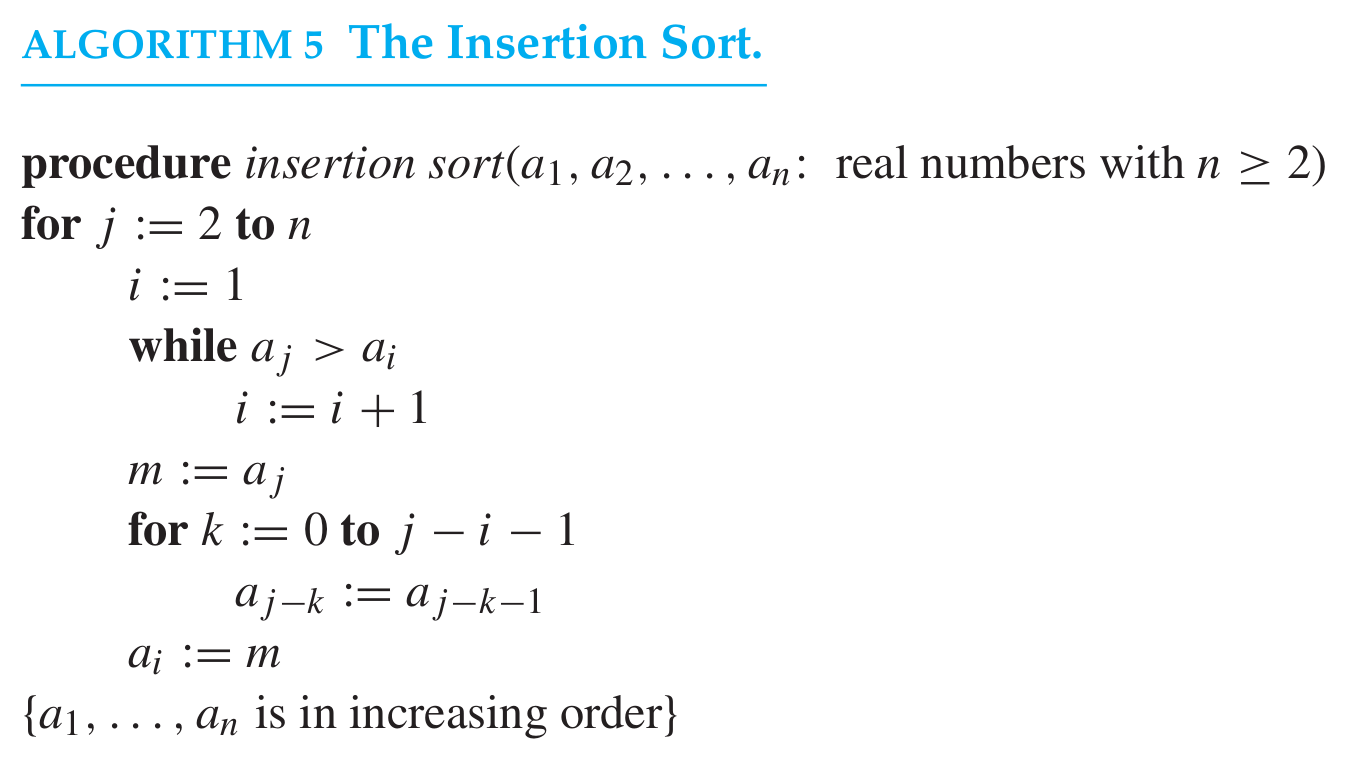
\includegraphics[width=\textwidth]{insertion-sort}
\end{center}
\end{frame}

\begin{frame}{Tímaflækja innsetningarröðunar}
\begin{itemize}
 \item Innsetningarröðun notar línulega leitaraðferð til að finna stað fyrir hvert stak \pause
 \begin{itemize}
  \item $O(n)$ tími
 \end{itemize}
 \item Öllum stökum er svo hliðrað \pause
 \begin{itemize}
  \item $O(n)$ tími
 \end{itemize}
 \item Þetta þarf að gera $n-1$ sinni
 \begin{itemize}
  \item Heildarkeyrslutími í versta tilfellinu $\Theta(n^2)$
 \end{itemize}
 \item Til eru almenn röðunarreiknirit sem virka á $\Theta(n\log(n))$ tíma
\end{itemize}
\end{frame}

\subsection{Fylkjamargföldun}

\begin{frame}{Fylkjamargföldun}
Skoðum reiknirit sem framkvæmir fylkjamargföldun á $m \times k$ fylkinu $A$ og $k \times n$ fylkinu $B$:
\begin{center}
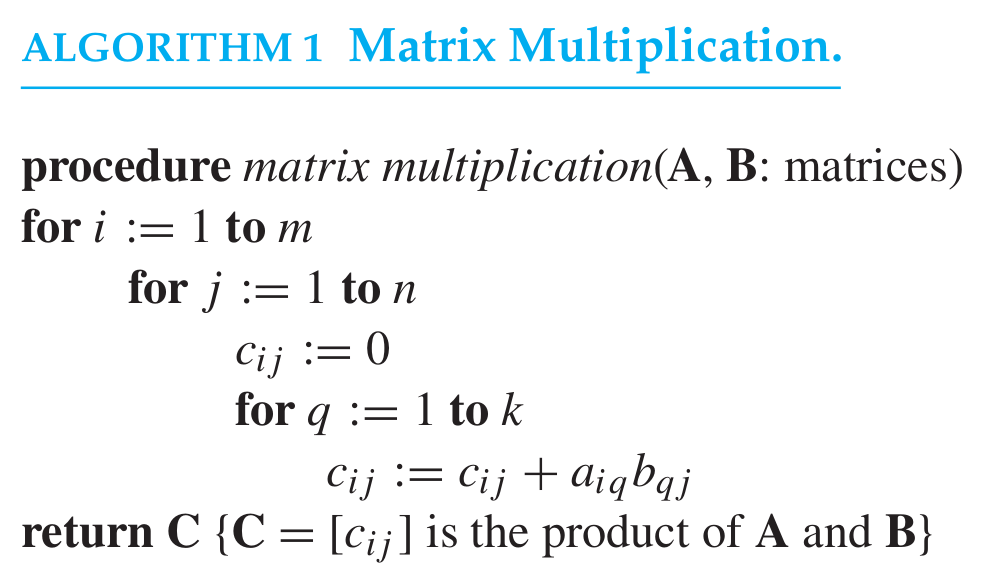
\includegraphics[width=0.8\textwidth]{matrix-multiplication}
\end{center}
\end{frame}

\begin{frame}{Tímaflækja fylkjamargföldunar}
\begin{itemize}
 \item Um er að ræða $m \cdot n$ stök, til að mynda hvert þeirra þarf $k$ samlagningar \pause
 \begin{itemize}
  \item Heildartímaflækja: $O(kmn)$
  \item Verður $O(n^3)$ þegar $m = n = k$ (tvö ferningsfylki)
 \end{itemize}\pause
 \item Til eru reiknirit með lægri tímaflækjur fyrir tvö ferningsfylki
 \begin{itemize}
  \item Strassen-reikniritið: $\approx O(2.81)$
  \item Coppersmith-Winograd reikniritið: $O(n^{2.375477}$)
  \begin{itemize}
   \item Nýrri útgáfur: $O(n^{2.374})$ (Stothers, 2010) \pause, $O(n^{2.3728642})$ (Williams, 2011), \pause $O(n^{2.3728639})$ (Le Gall, 2014)
  \end{itemize}
 \end{itemize}
\end{itemize}
\end{frame}

\begin{frame}{Tímaflækjur - raunveruleg áhrif}
Keyrslutími reiknirita á tölvu þar sem ein bitaaðgerð tekur $10^{-11}s$.
\begin{center}
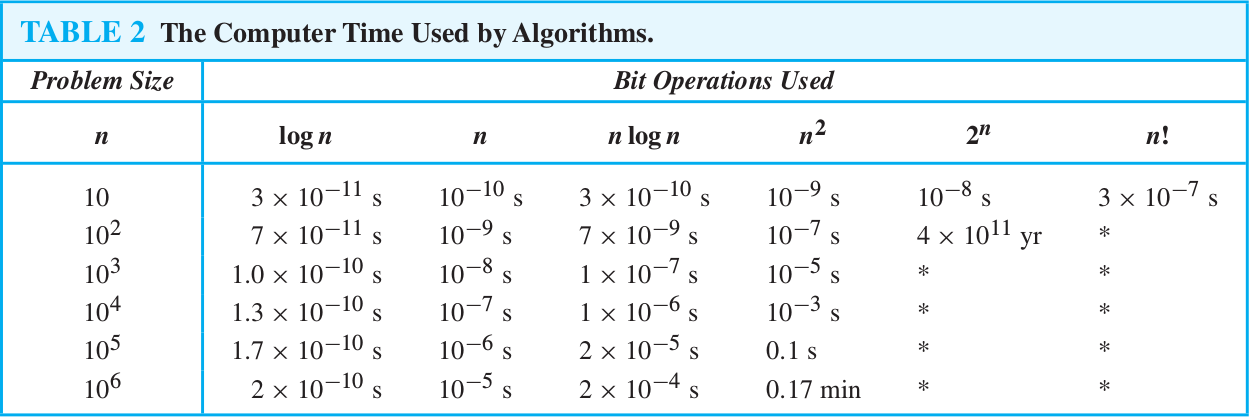
\includegraphics[width=\textwidth]{time-table}
\end{center}
Hér er $* > 10^{100}$ ár.
\end{frame}

\begin{frame}{Keyrslutímar - hugtök}
\begin{center}
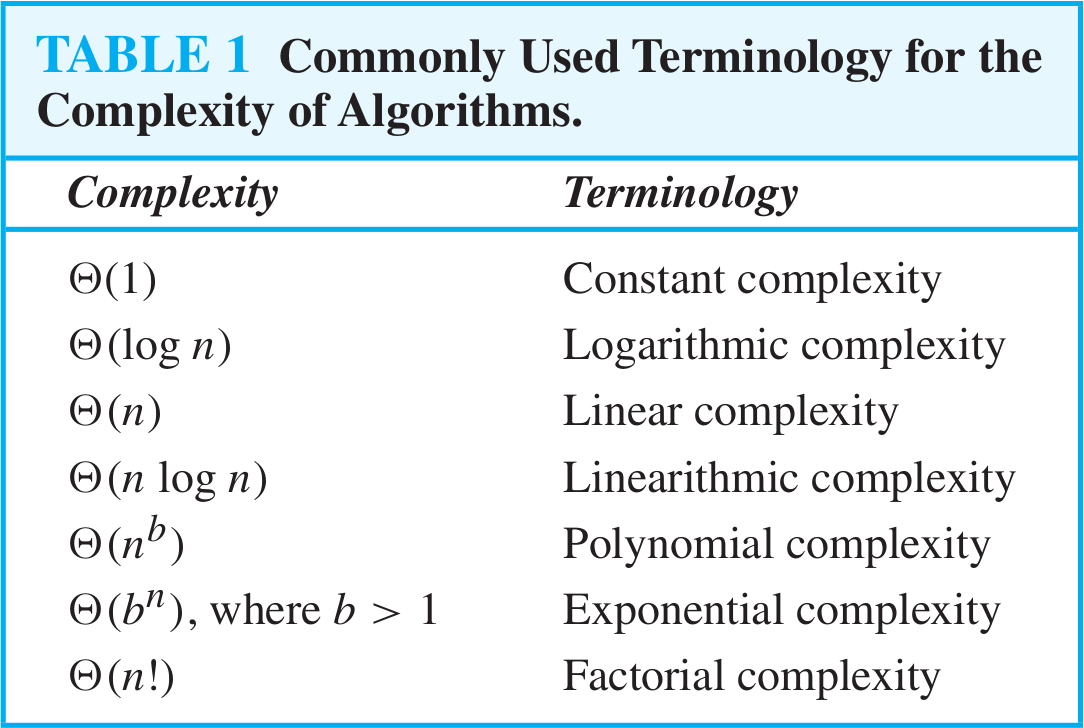
\includegraphics[width=\textwidth]{complexity-terminology}
\end{center}
\end{frame}


\section{P = NP}

\begin{frame}{Meðfærileiki vandamála}
\begin{itemize}
 \item Mjög mikill munur er á vexti veldisvísisfalla og margliða
 \item Skipta má vandamálum í meðfærileg (e. \emph{tractable}) og ómeðfærileg (e. \emph{intractable})
 \item Flest vandamál sem eru leysanleg með reikniriti sem keyrir á margliðutíma eru meðfærileg
 \begin{itemize}
  \item Leit í runu, röðun, fylkjamargföldun\ldots
 \end{itemize}
 \item Flest vandamál sem ekki hafa þekkt reiknirit sem leysir þau á margliðutíma eru ómeðfærileg
 \begin{itemize}
  \item Skák á $n \times n$ borði, stöðvast gefið forrit með gefið inntak í $k$ skrefum?
 \end{itemize}
\end{itemize}
\end{frame}

\begin{frame}{P og NP}
\begin{itemize}
 \item Sum vandamál eru þess eðlis að hægt er að leysa þau á margliðutíma í versta tilfellinu, mengi slíkra vandamála er kallað $P$
 \item Sum vandamál eru þess eðlis að hægt er að staðfesta eða hafna gefinni lausn á þeim á margliðutíma í versta tilfellinu, mengi slíkra vandamála er kallað $NP$
 \item Stærsta opna spurningin í tölvunarfræði:
\end{itemize}
\[
 \text{er } P = NP \text { eða } P \neq NP \text{ ? }
\]
\end{frame}

\begin{frame}{NP-complete vandamál}
\begin{itemize}
 \item $NP$-complete vandamál eru flokkur vandamála innan $NP$ sem hefur merkilegan eiginleika:
 \begin{itemize}
  \item Sé til reiknirit sem leysir eitthvert $NP$-complete vandamál á margliðutíma er til reiknirit sem leysir öll $NP$-vandamál á margliðutíma
 \end{itemize}
 \item Yfir 3000 þekkt $NP$-complete vandamál
 \item Fyrsta sannanlega $NP$-complete vandamálið var ``boolean satisfiability problem''
 \begin{itemize}
  \item Er til ákvörðun á $n$ rökbreytum svo að gefin yrðing sé sönn?
 \end{itemize}
\end{itemize}
\end{frame}

\begin{frame}{Samband mengjanna (Wikipedia)}
\begin{center}
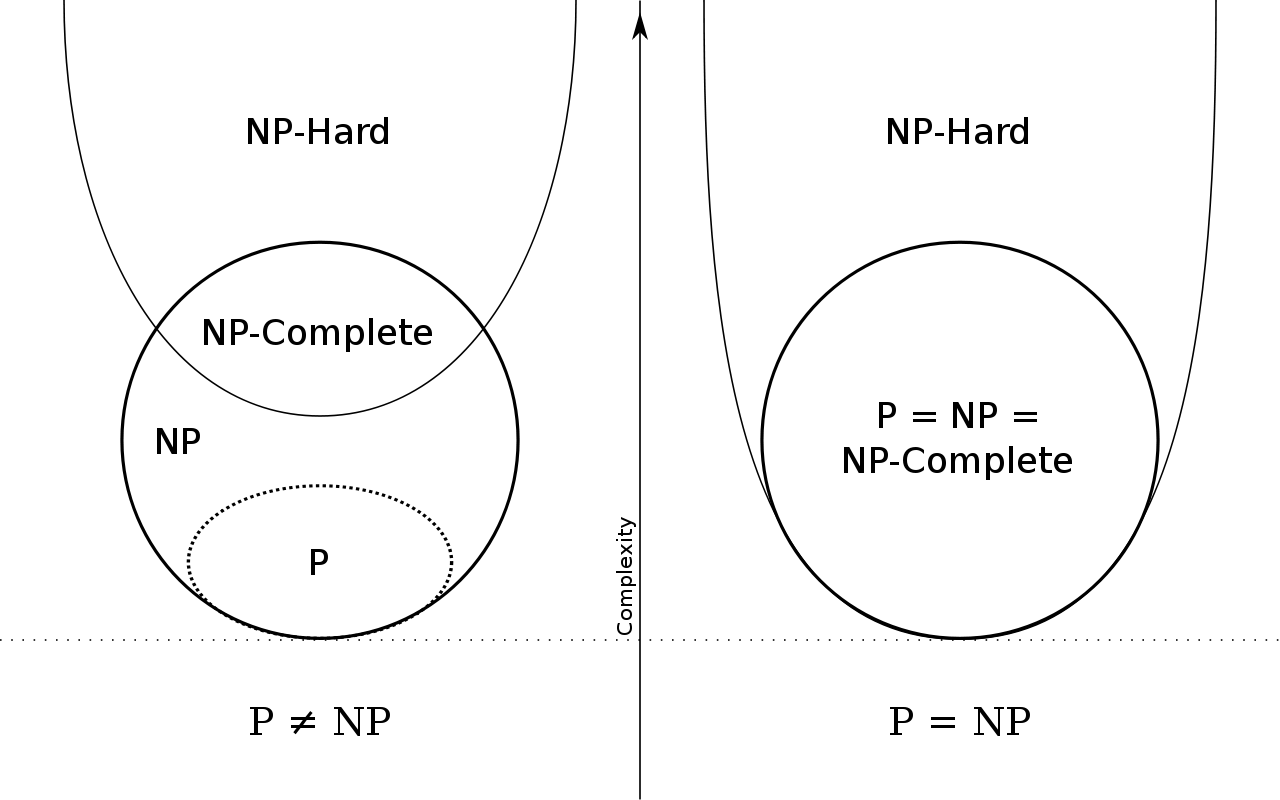
\includegraphics[width=\textwidth]{P-NP}
\end{center}
\end{frame}


\begin{frame}{Næst}
\begin{itemize}
 \item 4.1 (Deiling og deilingarafgangur)
 \item 4.2 (Mismunandi grunntölur)
 \item 4.3 (Prímtölur)
\end{itemize}

\end{frame}


\end{document}
